\documentclass{beamer}
 
\usepackage[american]{babel}
\usepackage[utf8]{inputenc}
\usepackage[T1]{fontenc}
\usetheme{Copenhagen}
\setbeamertemplate{navigation symbols}{}
%\title[Translittération automatique]{Données Séquentielles et Symboliques: Translittération automatique}
\title[Machine Transliteration]{Sequential Symbolic Data: Machine Transliteration}
\author[A.~Bérard, M.~Millet, C.~Robin]{Alexandre Bérard, Mathias Millet, Charles Robin}

\date{January 10th, 2014}

\newcommand*\oldmacro{}%
\let\oldmacro\insertshorttitle%
\renewcommand*\insertshorttitle{%
  \oldmacro\hfill%
  \insertframenumber\,/\,\inserttotalframenumber}

\begin{document}

\begin{frame}
\titlepage
\end{frame}

\section{Introduction}   
 
\begin{frame}
    \frametitle{Introduction}
	\framesubtitle{Translitération}
	\begin{block}{Definition}
	    Remplacement d'un graphème d'un système d'écriture par un ou plusieurs graphèmes d'un autre système d'écriture
    \end{block}	    
    
	\begin{exampleblock}{Examples : anglais - hindi}
	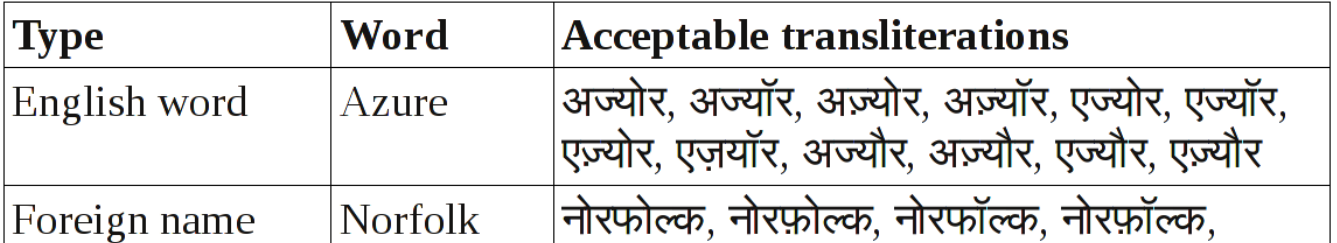
\includegraphics[scale=0.2]{en-in-example}
    \end{exampleblock}
    
	\begin{block}{Pourquoi ?}
	\begin{itemize}
		\item Traduction automatique de termes techniques
		\item Traduction automatique de requ\^etes
		\item Plus besoin de maintenir un dictionnaire !
	\end{itemize}
	\end{block}	    
    
    
\end{frame}

\begin{frame}
\frametitle{Introduction}
\framesubtitle{Le projet}

	\begin{block}{Le but}
		Implémenter des techniques de translitération 
		\begin{itemize}
		\item Entre l'espagnol et le portugais
		\item Entre l'anglais et le russe
		\end{itemize}
	\end{block}

	\begin{block}{Les données}
	Pour chaque pair de languages :		
		\begin{itemize}
		\item Un corpus d'apprentissage
		\item Un corpus de test
		\end{itemize}		
	\end{block}

\end{frame}

\section{Translittération}

\subsection{Méthodologie}

\begin{frame}
\frametitle{Méthodologie}

	\begin{block}{Échantillonage ?}
	Les données fournies sont déjà séparées entre données d'apprentissage et données de test\\
	$\Longrightarrow$ L'échantillonage n'est pas nécéssaire
	\end{block}

	\begin{block}{Métriques}
	Deux métriques  :
		\begin{itemize}
		\item Précision (distance binaire ????)
		\item Distance de levenstein : $d(x,y) = \min_{y' \in traductions(x)} \{\delta(y,y')\}$

où $\delta(y,y')=levenshtein(y,y')$
		\end{itemize}		
	\end{block}
\end{frame}

\subsection{Translittération par règles de substitution}


\begin{frame}[fragile]
	\frametitle{Espagnol - Portugais}

	\begin{block}{Premières considérations}
		\begin{itemize}
		\item Les deux langues sont très proches (51\% de précision sans rien faire)
		\item En appliquant les trois règles suivantes : {\scriptsize \begin{verbatim}
			is#->e#
			ción#->ção#
			ido#->ídeo#
			\end{verbatim}}
			nous obtenons 57\% de précision
		\end{itemize}
	\end{block}

	\begin{alertblock}{}
	$\Longrightarrow$ De bons résultat peuvent être obtenus en déterminant des règles automatiquement 
	\end{alertblock}
\end{frame}

\begin{frame}
	\frametitle{Apprentissage}

	\begin{block}{Objectif}
	Trouver un compromis entre :
		\begin{itemize}
		\item Fiabilité : la règle ne conduit pas à de fausses translitérations
		\item Généralisation : la règle peut s'appliquer à beaucoup de mots
		\end{itemize}			
	\end{block}

	\begin{block}{}
	
	\end{block}

\end{frame}


\begin{frame}
    \frametitle{Bibliography}
    {\fontsize{0.8em}{1em}
    \nocite{*}
    \bibliographystyle{plain}
    \bibliography{report}}
\end{frame}

\begin{frame}
    \frametitle{Overview}
\end{frame}

\section{Conclusion}
\begin{frame}
    \frametitle{Conclusion}
    \url{https://code.google.com/p/transliteration}
\end{frame}

\end{document}
